\subsection{\href{https://www.argentina.gob.ar/comision-nacional-de-energia-atomica}{Comisión Nacional de Energía Atómica}}
   \hypertarget{subsec:cnea}
   Se trabajó en la CNEA como becario de investigación en el grupo de
   desarrollo de un PET, Tomógrafo por Emisión de Positrones.\\
   Se desarrolló una mesa CNC para el movimiento a distancia de material
   radioactivo y en la codificación VHDL de las FPGA's del calculo de
   coincidencias de fotones mostrado en la figura \ref{fig:cnea1}.\\
   Luego se desarrolló el software de adquisición y análisis de datos
   crudos provenientes del equipo mostrado en la figura \ref{fig:cnea2}.
   \begin{figure}
      \begin{center}
         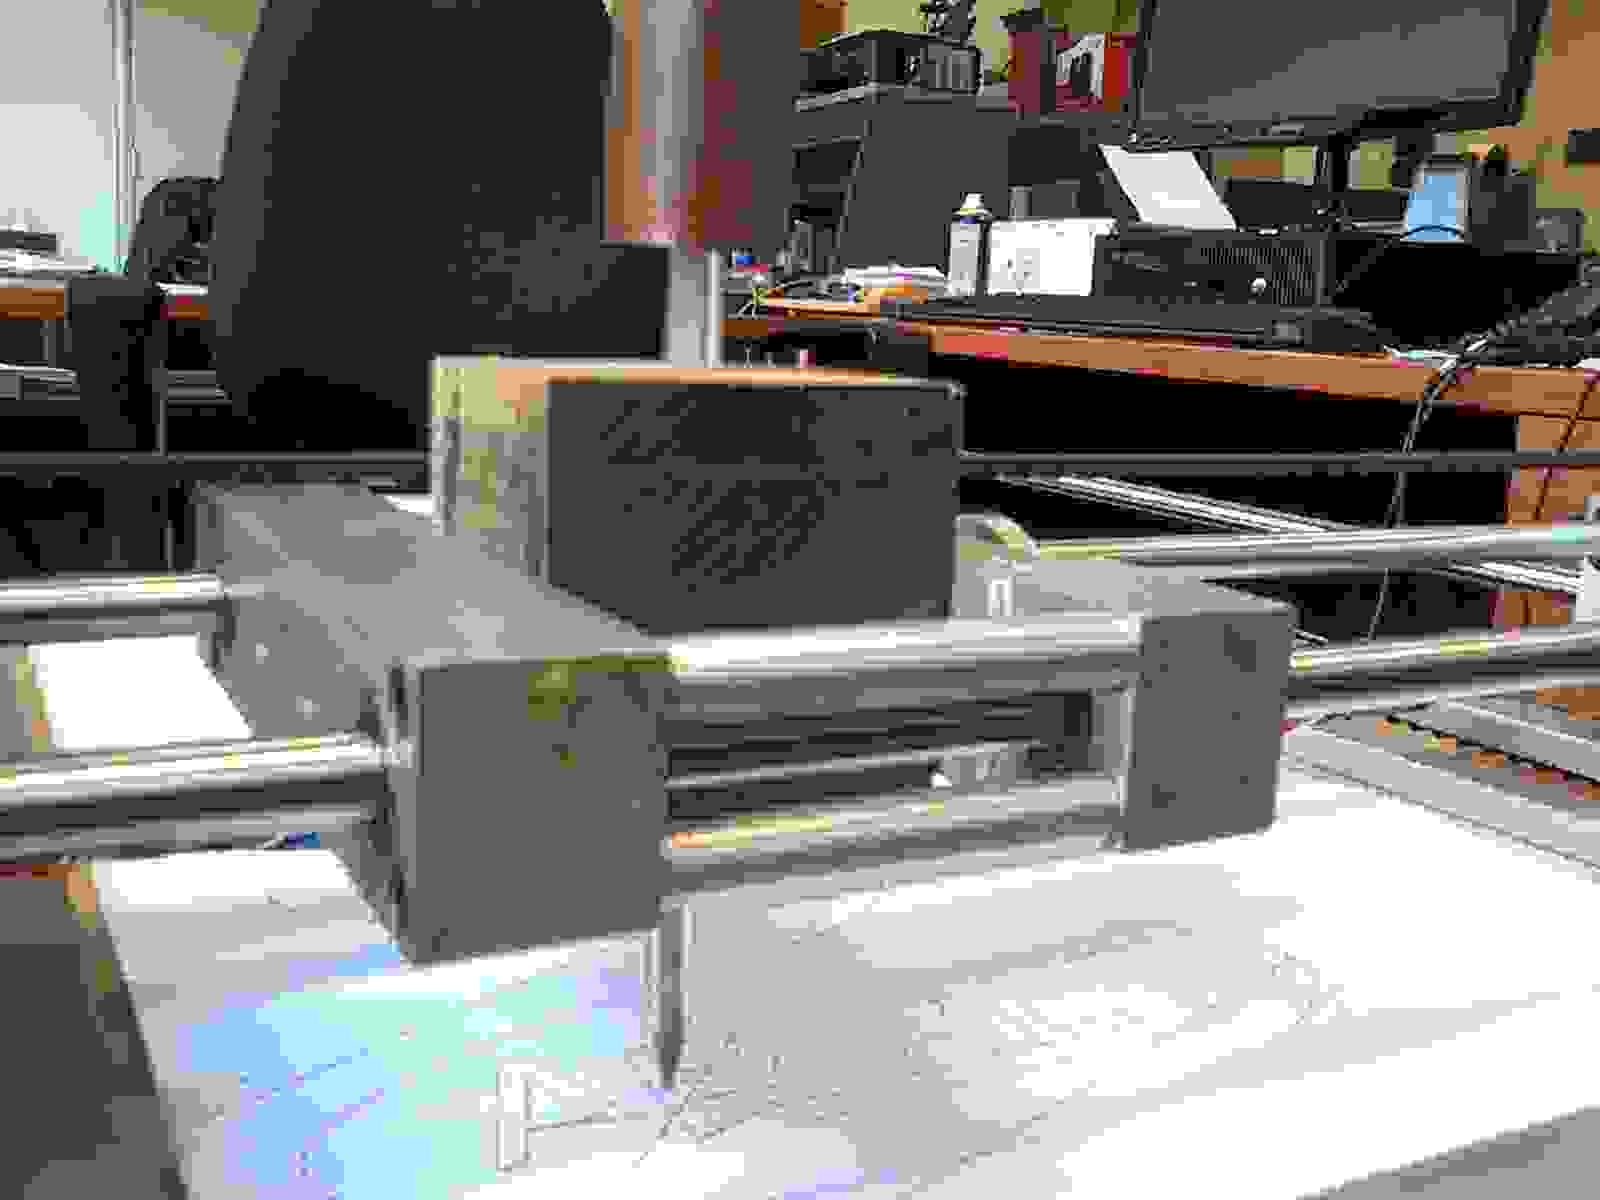
\includegraphics[width=0.24\textwidth]{portfolio/cnea_mesa1.jpg}
         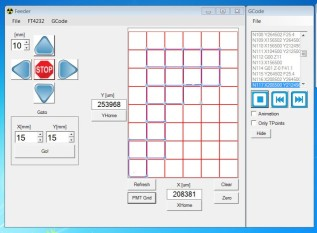
\includegraphics[width=0.24\textwidth]{portfolio/cnea_mesa2.jpg}
         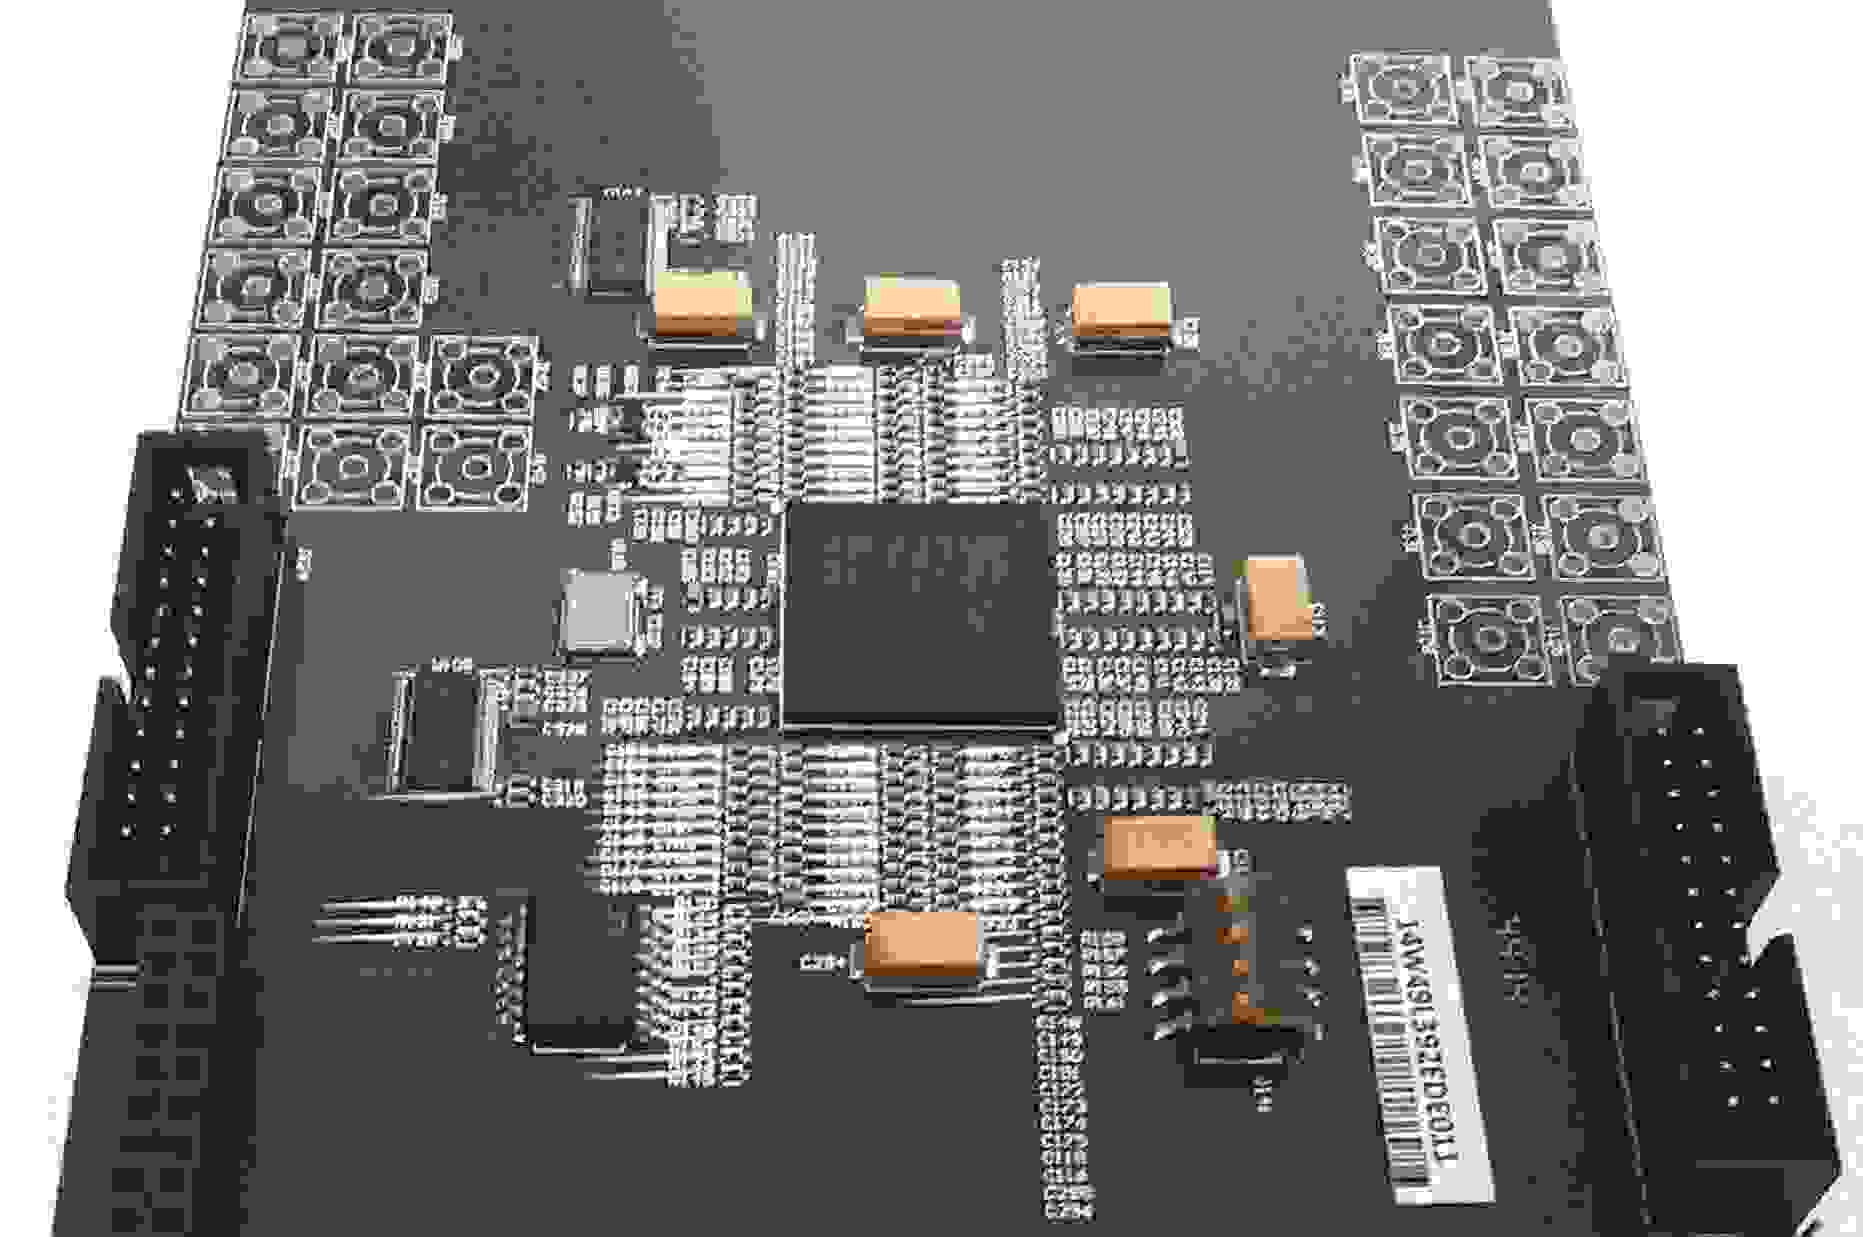
\includegraphics[width=0.24\textwidth]{portfolio/cnea_coin1.jpg}
         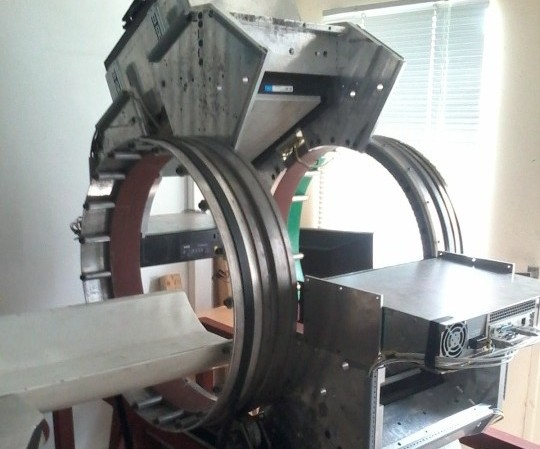
\includegraphics[width=0.24\textwidth]{portfolio/cnea_coin2.jpg}
      \end{center}
      \caption{Mesa CNC para automatización de adquisiciones con una captura del software de manejo, la placa con la FPGA montada en uno de los 6 cabezales, y el tomógrafo a medio armar.}
      \label{fig:cnea1}
   \end{figure}
   \begin{figure}
      \begin{center}
         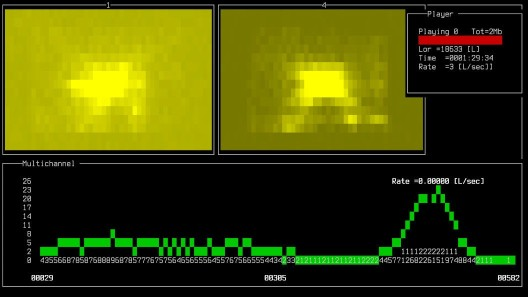
\includegraphics[width=0.24\textwidth]{portfolio/cnea_cuipet1.jpg}
         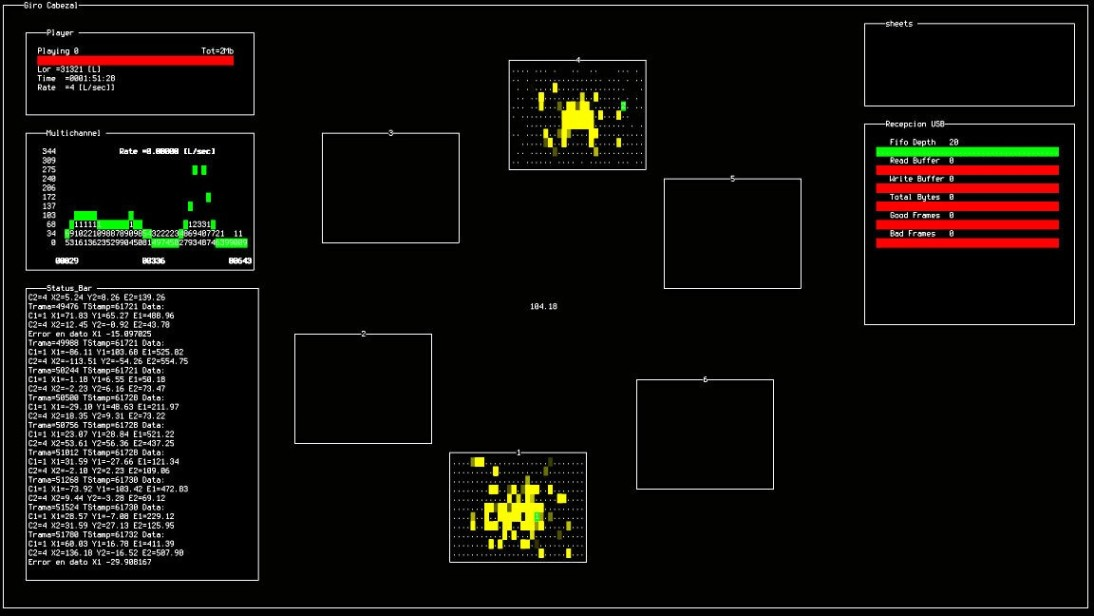
\includegraphics[width=0.24\textwidth]{portfolio/cnea_cuipet5.jpg}
         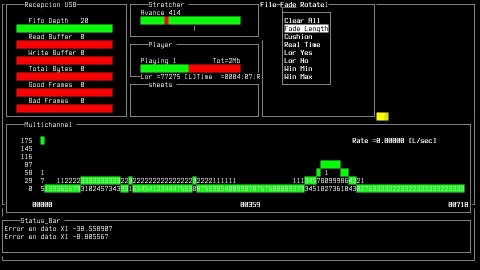
\includegraphics[width=0.24\textwidth]{portfolio/cnea_cuipet3.jpg}
         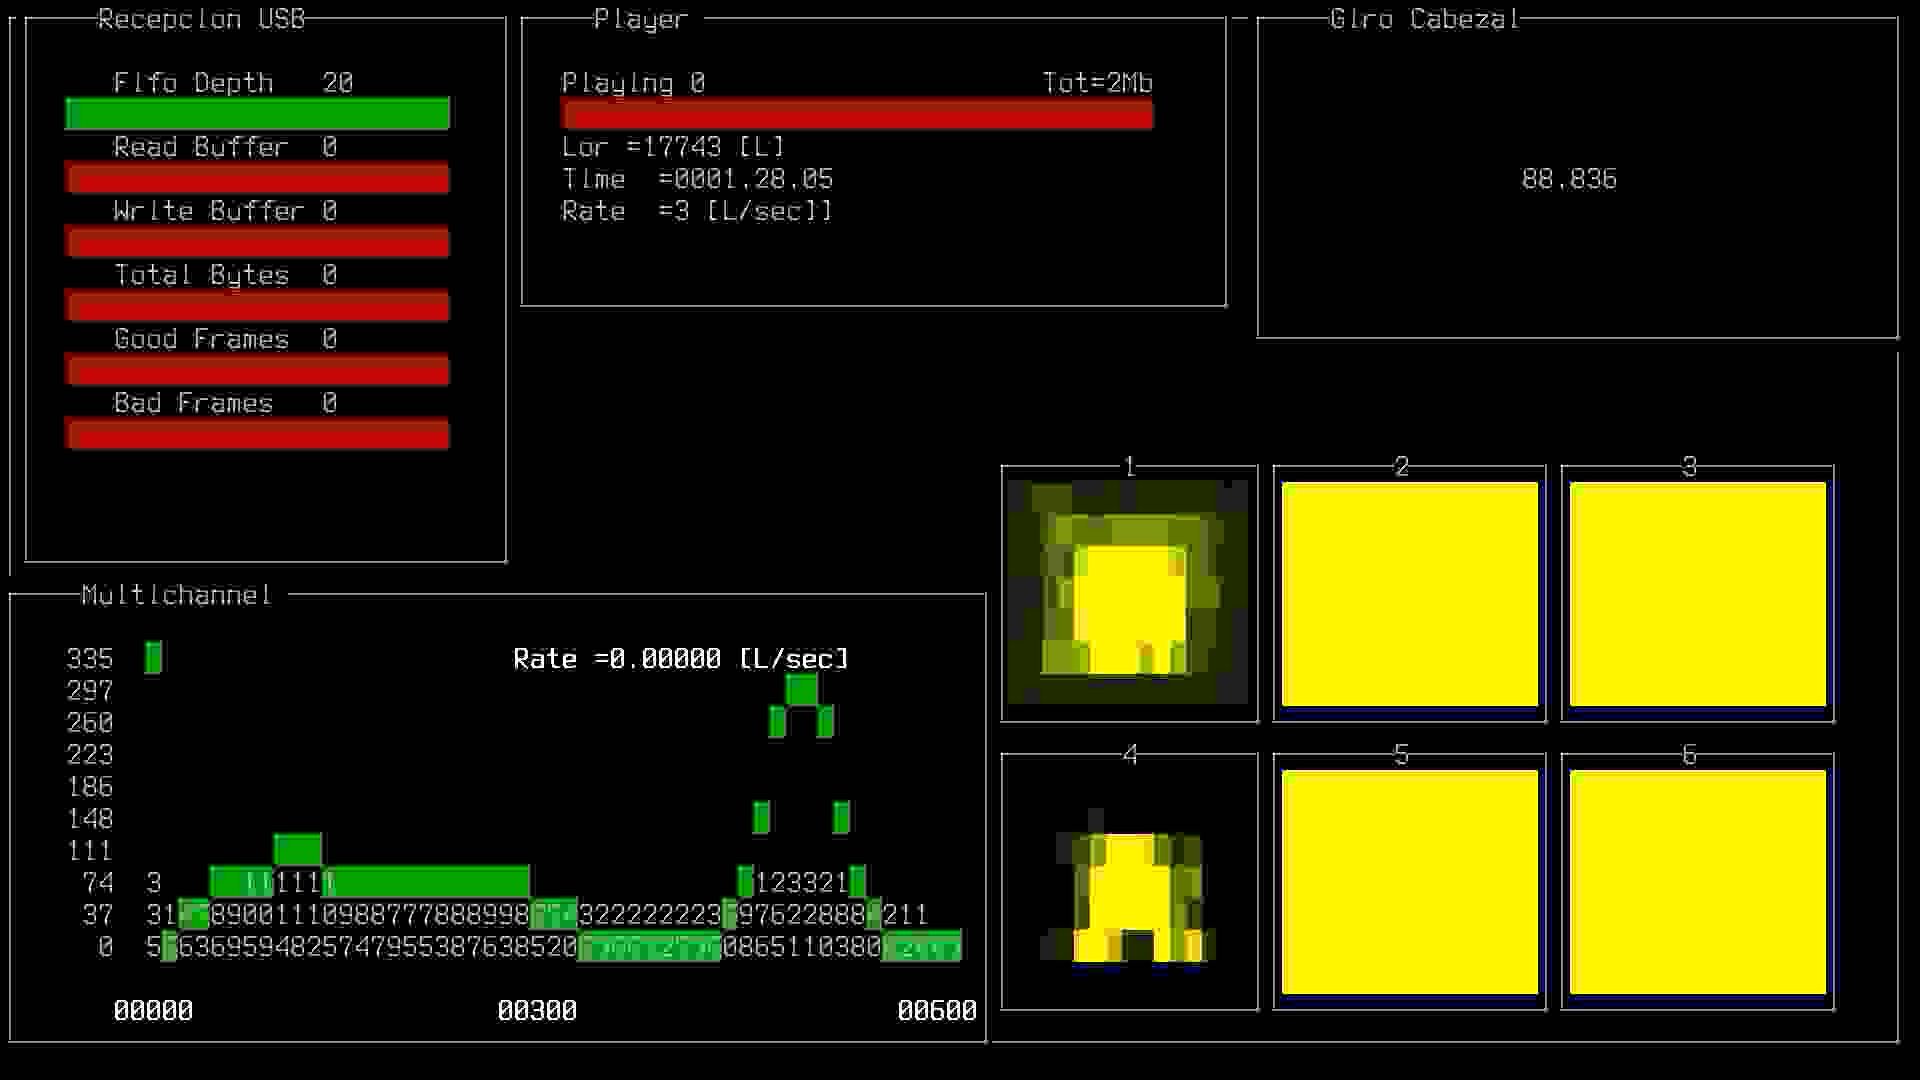
\includegraphics[width=0.24\textwidth]{portfolio/cnea_cuipet4.jpg}
      \end{center}
      \caption{Capturas del software de adquisición, CUIPET, del PET en la CNEA.}
      \label{fig:cnea2}
   \end{figure}
